\large \bf{\textsc{\section{Lab 4}}
	\begin{problem}
		Using an OpAmp TL082, construct an amplifier that can deliver the following functions. Evaluate your circuit practically and theoretically.
		\newline
		1. z = 0.2x + y\\
		2. z = 3(x-y)\\
	\end{problem}
	
	\begin{solution}
		1. 
		\newline
		2. z = 3(x-y)
		
		x = 5V, y = 3V => 2*3=6V
	\end{solution}
	\clearpage
	\begin{problem}
		We would like to investigate the properties of the MOSFET type BS170. Construct the following circuit with R=1K\(\Omega\). (a and b are equivalent)
		\begin{figure}[h!]
			\centering
			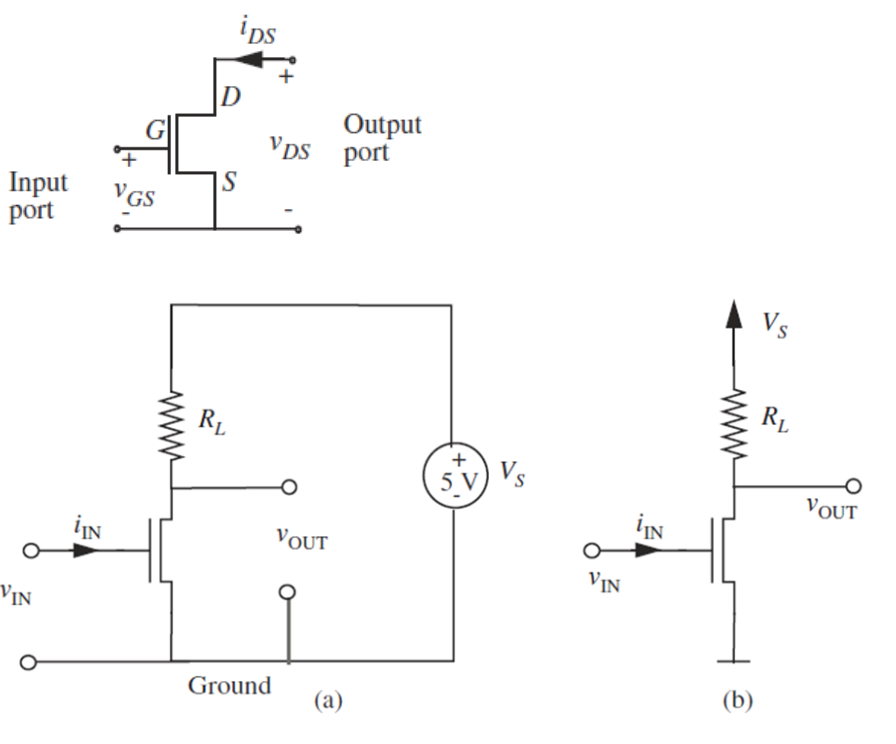
\includegraphics[width=0.4\textwidth]{images/circuit4.png}
		\end{figure}
		\newline
		1. Measure the V\(_{out}\) and i\(_{DS}\) for the MOSFET for different values of V\(_{IN}\) and fill the table.
		\newline
		2. Plot your input-output characteristics of the MOSFET. What is the treshold voltage V\(_{T}\) for V\(_{GS}\)? Compare your findings with the datasheet.
		\newline
		3. Measure the V\(_{DS}\) and i\(_{DS}\) for the MOSFET for different values of V\(_{S}\) and fill the table once the MOSFET is on.
		\newline
		4. Plot the I-V characteristics of the MOSFET and obtain R\(_{ON}\). Compare your findings with the datasheet.
	\end{problem}
	
	\begin{solution}
		1. 		
		\begin{table}[h]
			\begin{tabular}{| l | l | l | l | l | l | l | l | l | l | l | l |}
				\hline
				Try & 1 & 2 & 3 & 4 & 5 & 6 & 7 & 8 & 9 & 10 & 11 \\ \hline
				V$_{OUT}$ (V) & 5 & 5 & 4.965 & 4.827 & 3.980 & 1.090 & 0.057 & 0.025 & 0.019 & 0.010 & 0.008 \\ \hline
				V$_{IN}$ (V) & 0 & 1 & 1.9 & 2.1 & 2.3 & 2.5 & 2.7 & 2.9 & 3 & 4 & 5 \\ \hline
			\end{tabular}
		\end{table}
		\newline
		2.
		\begin{figure}[h!]
			\centering
			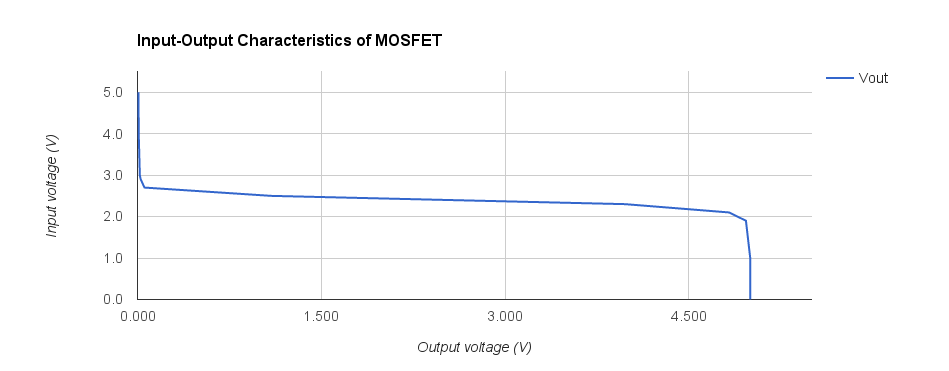
\includegraphics[width=0.8\textwidth]{images/plot422.png}
		\end{figure}
		3.
		\begin{table}[h]
			\begin{tabular}{| l | l | l | l | l | l | l | l | l | l | l | l |}
				\hline
				Try & 1 & 2 & 3 & 4 & 5 & 6 & 7 & 8 & 9 & 10 & 11 \\ \hline
				V$_{OUT}$ (V) & 0.008 & 0.010 & 0.011 & 0.013 & 0.014 & 0.016 & 0.018 & 0.019 & 0.021 & 0.022 & 0.024 \\ \hline
				V$_{S}$ (V) & 5 & 6 & 7 & 8 & 9 & 10 & 11 & 12 & 13 & 14 & 15 \\ \hline
				i$_{DS}$ (mA) & 5 & 6 & 7 & 8 & 9 & 10 & 11 & 12 & 13 & 14 & 15 \\ \hline
			\end{tabular}
		\end{table}
		\newline
		4.
		\begin{figure}[h!]
			\centering
			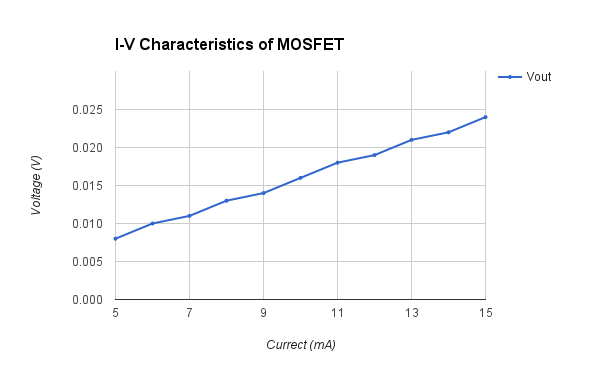
\includegraphics[width=0.8\textwidth]{images/plot424.png}
		\end{figure}
	\end{solution}
	\clearpage
	\begin{problem}
		Using MOSFET type BS170, construct circuits that represent the following logic functions. Evaluate your circuit practically and theoretically.
		\newline
		1. A+B+C \\
		2. A.B+\(\overline{C}\) \\
		3. A.B+C \\
		4. \(\overline{A.\overline{B}+\overline{C}}\)
	\end{problem}
	
	Solution.
